\chapter{Experiment: agent training and simulation}
Chapters 4 and 5 focus on the experimental phase of our project. This chapter details the training procedure of our SAC agent for the swing-up task and then transitions to a simulation phase to validate results for both the swing-up and stabilization tasks. We have structured this chapter into three distinct subsections: training setup, training process, and simulation results.

The first subsection describes the foundation of a reinforcement learning interaction rooted in a stable baseline3-based RL algorithm. It also touches upon a customized environment inherited from the OpenAI Gym environment. The second subsection centers on hyperparameter tuning and highlights the challenges encountered during training. The third subsection displays the results acquired from both the pendubot and acrobot setups.
\section{Training setup}
Stable Baseline 3(SB3)[some paper] is an open-source implementation of deep reinforcement learning algorithms based on the Python language. This library includes seven commonly used model-free deep reinforcement learning algorithms including SAC. Prior implementations of deep RL algorithms often encountered a problem wherein small implementation details could greatly affect performance, typically exceeding the differences between algorithms[some paper]. The developers of SB3 have done a commendable job stabilizing the performance of these deep RL algorithms by benchmarking each one on common environments and comparing them to prior implementations. Owing to its user-friendly and reliable nature, we chose Stable Baseline 3 as our RL library, which greatly simplified our research process.

OpenAI Gymnasium[some paper] is a toolkit for developing and comparing reinforcement learning algorithms, and it is widely used in the research community. Among its many advantages are its open-source nature and standardized environments, which facilitate the rapid testing and benchmarking of new algorithms. Additionally, it offers easy visualization and monitoring. Our decision to use the Gym library is based on its extensibility—from standard environments to highly customized ones—as well as its capability to integrate with tools like PyTorch and TensorFlow for GPU-accelerated computations. Furthermore, Gym provides the ability to construct stacked training environments for parallel training.

\begin{figure}[htbp]
    \centering
    \includegraphics[width=0.7\linewidth]{example-image}
    \caption{Interaction between reinforcement learning agent and customized environment}
    \label{fig:my_label}
\end{figure}

To construct the customized environment, we begin with the symbolic dynamic function that captures the nonlinear dynamics of the underactuated double pendulum. This function uses the current state observation from the simulation and the action determined by the control policy, producing a prediction of the next state via a Runge-Kutta integrator.

This predicted state is then input into the reward function, which yields a scalar output. This output is subsequently relayed to the SAC algorithm for policy evaluation and update. After these computations, the simulation provides an estimation of the current state, and the policy identifies the most probable action. Both of these values are then directed back to the dynamics function, initiating a new cycle.

It's widely recognized \cite{some paper} that reinforcement learning algorithms tend to converge more effectively when using normalized state and action spaces. Therefore, we've designed a scaling mechanism to translate the state and action spaces from their normalized versions to real-world measurements. Users can choose to activate or deactivate this scaling. For example, while a normalized state resides within the interval \( [-1,1] \), we might wish to map it to real-world measurements \( \left[ \text{pos1}, \text{pos2}, \text{vel1}, \text{vel2} \right] \), such as \( \text{pos1} \) in \( [0,2\pi] \), \( \text{pos2} \) in \( [-\pi,\pi] \), and velocities \( \text{vel1} \) and \( \text{vel2} \) in \( [-20,20] \) rad/s, while keeping the torque within \( [-\tau_{\text{limit}}, \tau_{\text{limit}}] \). When this scaling mechanism is activated, it ensures that states and actions in the SAC algorithm always stay within the \( [-1,1] \) boundary, which often leads to faster convergence. The mapping relation of the scaling mechanism is demonstrated in the picture below:

\begin{figure}[H]
    \centering
    \includegraphics[width=0.7\linewidth]{example-image}
    \caption{mapping relation of the scaling mechanism}
    \label{fig:my_label}
\end{figure}

The logic of the pipeline of the interaction of customized environment is described in the picture below.

\begin{figure}[H]
    \centering
    \includegraphics[width=0.7\linewidth]{example-image}
    \caption{logic of the interaction}
    \label{fig:my_label}
\end{figure}

\section{Training phase}
The training phase commenced immediately after we finished setting up the training pipeline. During the training of the SAC controller for both the acrobot and pendubot, our primary emphasis was on tuning several key hyperparameters. These encompassed the learning rate, control frequency, episode length, and learning timestep. We invested considerable effort in adjusting hyperparameters for the reward function and the LQR controller, given their pivotal roles in the learning process, as detailed in Table 4.1.

We set the learning rate at 0.01 to promote effective learning and adaptation. Additionally, we configured the control frequency of the simulation to 100Hz, ensuring frequent updates and heightened responsiveness in the control process. We selected an episode length of 1000 for both the Acrobot and Pendubot, translating to 10-second-long episodes, to provide sufficient exploration and learning opportunities. To harness the full training potential, we executed a total of 2e7 learning time steps for the pendubot and 5e7 for the acrobot, allowing the agent to accumulate vast experience and enhance its performance.


\begin{table}[H]
  \centering
  \begin{tabular}{p{2cm} | p{3cm} | p{3cm} | p{3cm}}
  Robot & Quadratic Reward  & Constant Reward & LQR\\
  \hline
  \multirow{5}{*}{Pendubot} & \(Q_1\) = 8.0  &  & \(Q_1\) = 1.92\\
  & \(Q_2\) = 5.0  & \(r_{line}=500\) & \(Q_2\) = 1.92\\
  & \(Q_3\) = 0.1  & \(r_{vel}=0.0\) & \(Q_3\) = 0.3\\
  & \(Q_4\) = 0.1  & \(r_{LQR}=1e4\)& \(Q_4\) = 0.3\\
  & \(R\) = 1e-4  & & \(R\) = 0.82\\
  \hline
  \multirow{5}{*}{Acrobot} & \(Q_1\) = 10.0  &  & \(Q_1\) = 0.97\\
  & \(Q_2\) = 10.0  & \(r_{line}=500\) & \(Q_2\) = 0.93\\
  & \(Q_3\) = 0.2  & \(r_{vel}=1e4\) & \(Q_3\) = 0.39\\
  & \(Q_4\) = 0.2  & \(r_{LQR}=1e4\) & \(Q_4\) = 0.26\\
  & \(R\) = 1e-4  &  & \(R\) = 0.11\\
  \end{tabular}
 \caption{Hyper parameters used for the SAC training and the LQR controller.}
 \label{tab:parameters}
\end{table}

The learning curve for a total of 2e7 timesteps for the pendubot is illustrated below.As depicted in the figure, from 0 to 1e7 timesteps, the learning curve experiences a gradual ascent. Between 1e7 and 1.2e7 timesteps, the learning curve surges rapidly, peaking in reward around one million. After 1.2e6 timesteps, the curve begins to stabilize with occasional fluctuations, and no substantial increase in reward is observed.

\begin{figure}[H]
    \centering
    \fbox{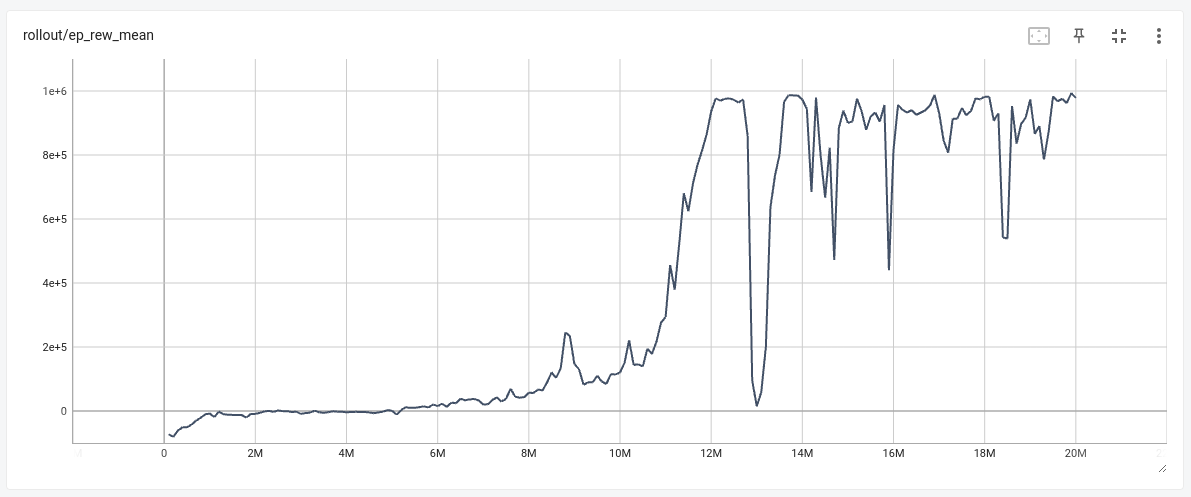
\includegraphics[width=0.9\textwidth]{figures/learning_curve/pendubot_learning_curve.png}} % First image
    \caption{pendubot learning curve}
    \label{fig:image_a}
\end{figure}

As shown in the learning curve over a total of 3e7 timesteps for the acrobot, the curve experienced a relatively steady growth until 1.8e7 timesteps. After a sudden drop in reward between 1.8e7 and 2e7 timesteps, the learning curve began to increase drastically, with two major fallbacks. By 3e7 timesteps, the learning curve hadn't reached its peak. We extended the learning period to 5e7 using a warm start from the model obtained at 3e7 timesteps, and the learning curve began to stabilize around 4e7 time steps.

\begin{figure}[H]
    \centering
    \fbox{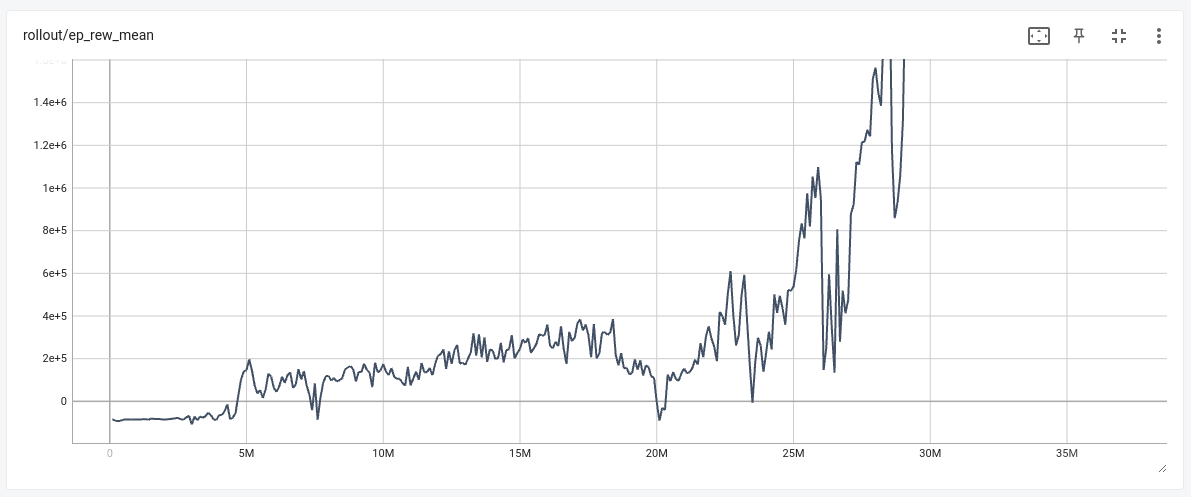
\includegraphics[width=0.9\textwidth]{figures/learning_curve/acrobot_learning_curve.png}} % Second image
    \caption{acrobot learning curve}
    \label{fig:image_b}
\end{figure}

\section{Simulation results}
This section is about simulation results in pendubot and acrobot.
\subsection{Pendubot simulation in ideal environment}
pendubot:
\begin{figure}[H]
    \centering
    \fbox{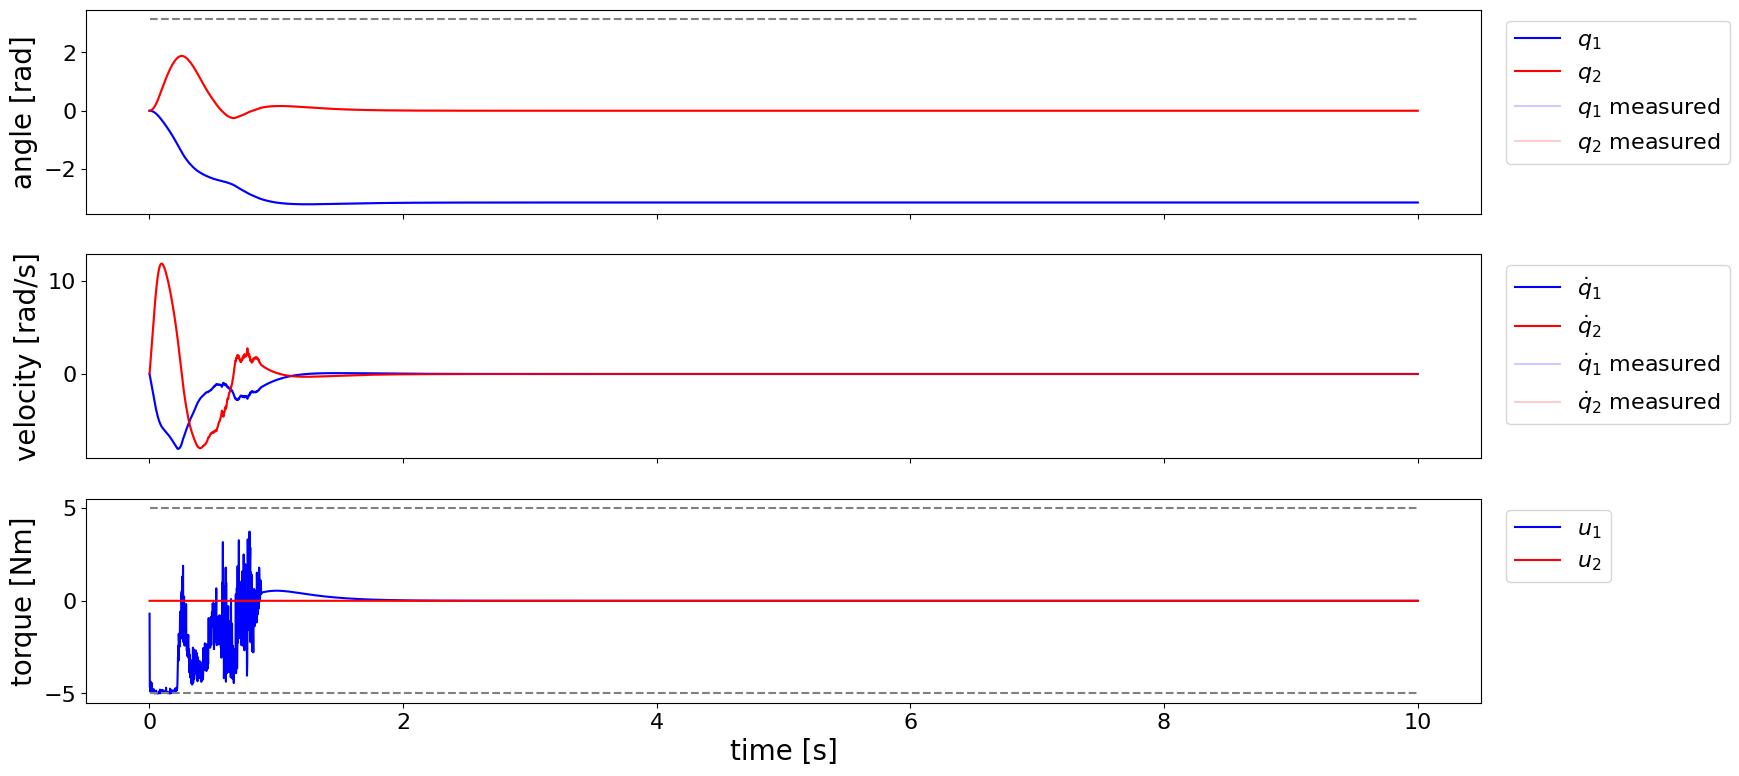
\includegraphics[width=0.9\textwidth]{figures/simulation_result/pendubot_unclipped.png}} % First image
    \caption{pendubot simulation result}
    \label{fig:image_a}
\end{figure}

\subsection{Acrobot simulation in ideal environment}
acrobot:
\begin{figure}[htbp]
    \centering
    \fbox{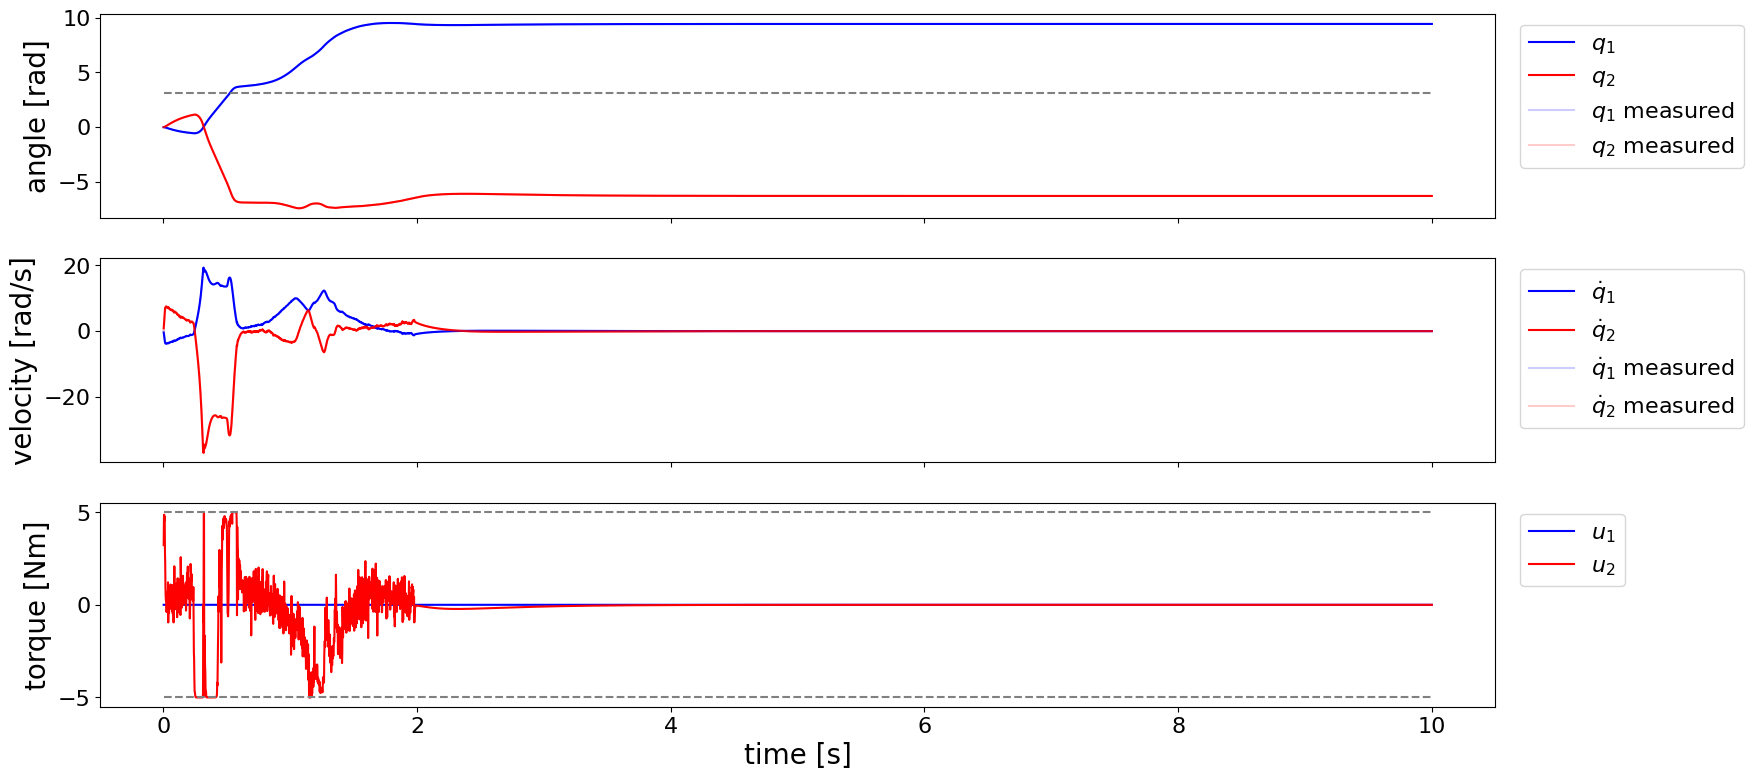
\includegraphics[width=0.9\textwidth]{figures/simulation_result/acrobot_unclipped.png}} % Second image
    \caption{acrobot simulation result}
    \label{fig:image_b}
\end{figure}


\cleardoublepage
